\title{Computational Photography}
\author{
        Assignment 5 - Hough Transform\\
Winter 2024
}
\date{}
\documentclass[12pt]{article}
\usepackage[margin=0.7in]{geometry}
\usepackage{graphicx}
\usepackage{float}
\usepackage{amsmath}


\begin{document}
\maketitle


\section*{Introduction}
In this assignment you will demonstrate your ability to implement utilize the \emph{Hough Transform} for finidng parameterizable objects from edge pixels.  In particulater, you will demonstrate your ability to:
\begin{itemize}
\item Generate ``fake'' edge data.
\item Apply hough transform to edge data for various parameterizable shapes.
\item Find local maxima in hough transform.
\item Generate shapes based on parameterized shapes.
\end{itemize}

\noindent
In this assignment, as with all of our assignments, you shouldn't be using built-in functions that violate the ``spirit'' of the assignment.  For instance, any sort of functions to generate circles or lines, or to compute hough transforms, are forbidden.  \emph{However}, since we have already implemented edge detection in a prior assignment, you \textbf{may} use a function like \emph{edge} to obtain edge pixels in an image.  In general, use your intuition, and when in doubt ask the instructor or TA.\\

\section*{Grading}
\begin{table}[h]
\begin{centering}
\begin{tabular}{|l|l|}
\hline
Theory Questions & 10pts \\
Generating lines and circles & 10pts\\
Hough transform for a line & 25pts\\
Hough transform for a circle & 25pts\\
Single circle detection on real image & 30pts\\
(Extra Credit) Multiple circle detection on real image & 10pts\\

\hline
\textbf{TOTAL} & 100pts\\
\hline
\end{tabular}
\caption{Grading Rubric}
\end{centering}
\end{table}

\newpage
\section*{Dataset}
For this assignment we're going to use two pieces of data:
\begin{enumerate}
\item Synthetically generated data
\item A provided grayscale image,  \emph{circles1.gif}
\end{enumerate}

\newpage
\section{Theory Questions}
\noindent
For the following questions, show the computations to support your answers.
\begin{enumerate}
\item (5pts) Given an image with a width of 200 pixels, and a height of 100 pixels, what is the size of the hough transform accumulator for lines if the step side for each parameter is 1.0 (assume that the angle is in degrees)?
\item (5pts) If the probability of an edge pixel is actually on the object we are attempting to detecting is $0.2$, and the desired accuracy of our model is $0.99$, how many independent tests must we run \emph{RANSAC} on, if we are attempting to detect a line?
\end{enumerate}


\newpage
\section{Generate Fake Data}
To start off with, let's generate some fake edge data so that we know what the ``solution'' is.\\

\noindent
Create a $400\times400$ binary image that has two objects on it:
\begin{itemize}
\item A line with slope $m=1$ and y-intersept $b=-100$.
\item A circle with center $x=100, y=200$ and radius $r=50$.
\end{itemize}

\noindent
You can generate the line by starting varying $x$ from its minimium to maximum value, generating $y$ values along the way according to the formula $y=mx+b$.\\

\noindent
You can generate the circle by varying $\theta =[0,2\pi]$ and generating the $(x,y)$ coordinates according to:
$$x =x_0 + rcos\left(\theta\right)$$
$$y=y_0 + rsin\left(\theta\right)$$
where $(x_0,y_0)$ is the center of the circle and $r$ is its radius.\\


\noindent
 \emph{Note} that since the origin of an image's coordinate system is the top-left, its positive y-axis is \emph{down}, and therefore your image is a reflection about the x-axis from what you might imagine it to be.

 
\newpage
\section{Hough Transform for a Line}
Next let's try to find the parameters of that line!  Apply the \emph{Hough Transform for a Line} to your binary image.  Use the \emph{polar} form, varying the of the parameters $\theta, r$ according to the slides, and incrementing them by one for each bin.\\

\noindent
\textbf{NOTE}:  You CANNOT use the Matlab function \emph{hough} or anything related to do this for you.  However, you MAY want to use a function like \emph{ind2sub} to help you get subscript indices from a linear index.\\

\noindent
In your report, provide:
\begin{itemize}
\item The value of $(\theta, r)$ that cooresonds to the maximum value in the Hough Transform.
\item The corresponding values for $(m,b)$ where $m$ is the slope and $b$ is the y-intercept.  Show the equations/formulas that allow you to compute those from $(\theta,r)$.
\item A plot of the Hough Transform as an image.
\end{itemize}


\newpage
\section{Hough Transform for Circle}
Next let's try to find that circle!  To find all the parameterize your circle, you'll need a 3D Hough Transform ($x_0, y_0, r$, where $x_0$ and $y_0$ are the $x$ and $y$ coordinates of the center of the circle, respectively, and $r$ is its radius).\\

\noindent
You may make the following assumptions:
\begin{itemize}
\item The circle's center is within the bounds of the image.
\item The circle's radius is less than the diagonal length of the image.
\end{itemize}

\noindent
Much like with the line, in your report, provide:
\begin{itemize}
\item The value of $(x_0, y_0, r)$ that cooresonds to the maximum value in the Hough Transform.
\item A plot of the Hough Transform as an image. \textbf{However}, since this is a 3D histogram just plot $x$ vs $y$ for the \emph{slice} where $r=rmax$ where $rmax$ is the value of $r$ find in the max bin.
\end{itemize}


\newpage
\section{Apply to a Real Image}
Now let's apply this stuff to a real image!\\

\noindent
For the problem we'll use the provide image \emph{circles.gif}.  However, this is a grayscale image, not a binary image.  In your previous assigment you implemented elements of a Canny Edge Detector.  For this one you'll just use Matlab's \emph{edge} function to do this for you.  Feel free to play with any parameters of that function, but if you deviate from the defaults, put in your report what parameters you changed.\\

\noindent
Once you have your binary image, apply your Hough Circle detection to it.   Display as subplots:
\begin{itemize}
\item Original image
\item Binary image
\item Original image with dominant circle superimposed in \emph{red}.
\end{itemize}


\noindent
Iin your report, provide:
\begin{itemize}
\item The value of $(x_0, y_0, r)$ that cooresonds to the maximum value in the Hough Transform.
\item The subplot image described earlier.
\end{itemize}


\newpage
\section{Extra Credit:  Additional Circles}
Of course there was more than one circle in that image!  For the last part, attempt to identify all the coins in the image (and nothing else).  To do this:

\begin{enumerate}
\item Apply a threshold to all the bins, such that any bin below the threshold is not considered a potential circle.
\item Apply \emph{3D non-maximum suppression} to the remaining candidates.  You \textbf{CANNOT} use a function like \emph{findlocalmaxima} or related.  You must do so yourself.
\end{enumerate}


\noindent
In your report provide a subplot like you did in the previous part as well as the parameters of the circles/coins you detected. 


\newpage
\section*{Submission}
For your submission, upload to Blackboard a single zip file containing:

\begin{enumerate}
\item PDF writeup that includes:
\begin{enumerate}
\item Your answer to the theory question(s).
\item For Part 2, your generated binary image.
\item For Part 3, the values for $\theta$ and $r$ that provide the maximum in your Hough transform, their corresponding values for the slope and y-intercept of that line, and an image of the Hough transform.
\item For Part 4, the values for the center and radius of the circle that provides the maximum in your Hough transform as well as an image of a \emph{slice} of the Hough transform where $r$ has its maximum value.
\item For Part 5, three images:  original image, binary edge image, and original image with detected dominent circle superimposed on it.  In addition, provide the parameters of that dominant circle.
\item For Part 6, (if applicable) A list of the parameters of the detected circles, the subplot image, similar to in the previous part.
\end{enumerate}
\item A README text file (\textbf{not} Word or PDF) that explains:
\begin{enumerate}
\item Any unique features of your program (if applicable).
\item Any instructions on how to run your script to reproduce your results.
\end{enumerate}
\item Your source file(s).
\end{enumerate}
\clearpage

\part{Answer to Theory Questions}
For the following questions, show the computations to support your answers.
\begin{enumerate}
	\item (5pts) Given an image with a width of 200 pixels, and a height of 100 pixels, what is the size of the hough transform accumulator for lines if the step side for each parameter is 1.0 (assume that the angle is in degrees)?
	\item (5pts) If the probability of an edge pixel is actually on the object we are attempting to detecting is $0.2$, and the desired accuracy of our model is $0.99$, how many independent tests must we run \emph{RANSAC} on, if we are attempting to detect a line?
\end{enumerate}

Given:
\begin{itemize}
	\item Image width = 200 pixels
	\item Image height = 100 pixels
	\item Step size for each parameter = 1.0
\end{itemize}

Steps:

\begin{enumerate}
	\item Calculate the range for \(\theta\). \(\theta\) ranges from 0 to 180 degrees, giving 181 possible values.
	
	\item Calculate the maximum distance \(r_{\text{max}}\):
	\[r_{\text{max}} = \sqrt{\left(\frac{200}{2}\right)^2 + \left(\frac{100}{2}\right)^2} = \sqrt{10000 + 2500} = \sqrt{12500} = 111.8\]
	
	\item Determine the range for \(r\). \(r\) can take values from -112 to 112, yielding 225 possible values.
	
	\item Calculate the size of the Hough transform accumulator:
	\[181 \times 225 = 40725\]
\end{enumerate}

Thus, the size of the Hough transform accumulator for lines is 40725.
Given the parameters:
\begin{itemize}
	\item Probability that a pixel is on the object, \(p = 0.2\),
	\item Number of pixels needed for our model, \(D = 2\) (for a line),
	\item Desired probability of success, \(P = 0.99\).
\end{itemize}

We use the RANSAC formula to calculate the number of independent tests (\(N\)) required:
\[1 - P = (1 - p^D)^N\]

Solving for \(N\), we get:
\[N = \frac{\log(1 - P)}{\log(1 - p^D)}\]

Substituting the given values into the formula:
\[N = \frac{\log(1 - 0.99)}{\log(1 - (0.2)^2)}\]

After performing the calculation, we find:
\[N \approx 112.811044\]
\[N \approx 113\]

Thus, to achieve a 99\% probability of successfully detecting the model, approximately 113 independent tests are required using the RANSAC method.

\clearpage
\part{Part 2-6 Images}


\begin{figure}
	\centering
	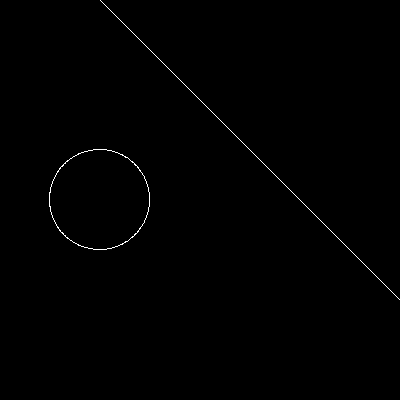
\includegraphics[width=0.7\linewidth]{binaryImage}
	\caption{Part 2 - Generated Binary Image.}
	\label{fig:binaryimage}
\end{figure}

\begin{figure}
	\centering
	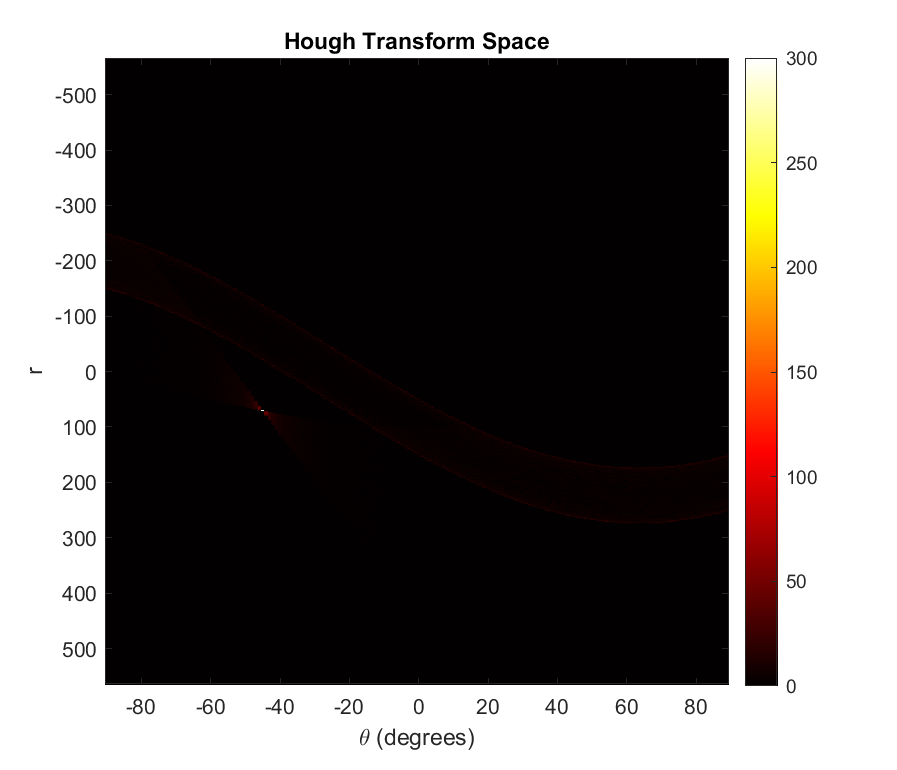
\includegraphics[width=0.7\linewidth]{HoughSpace}
	\caption{Part3 - Image of the Hough transform.}
	\label{fig:houghspace}
	\text Detected line: y = -1.04x + -101.22
	Detected Line Parameters:
	Theta (degrees): -136.00
	R: 70.31
	Slope (m): -1.04
	Y-intercept (b): -101.22
\end{figure}

\begin{figure}
	\centering
	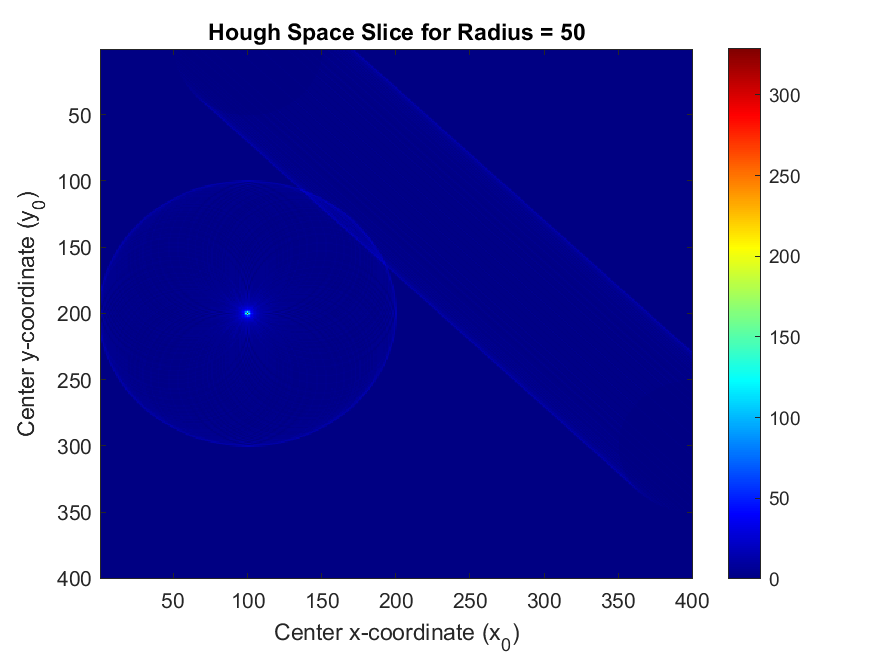
\includegraphics[width=0.7\linewidth]{houghSpaceSlice}
	\caption{Part 4 - Image of a \emph{slice} of the Hough transform where $r$ has its maximum value.}
	\label{fig:houghspaceslice}
	\text Detected Circle Parameters:
	Center: (100, 200)
	Radius: 50
	Maximum value in Hough Space: 329
\end{figure}


\begin{figure}
	\centering
	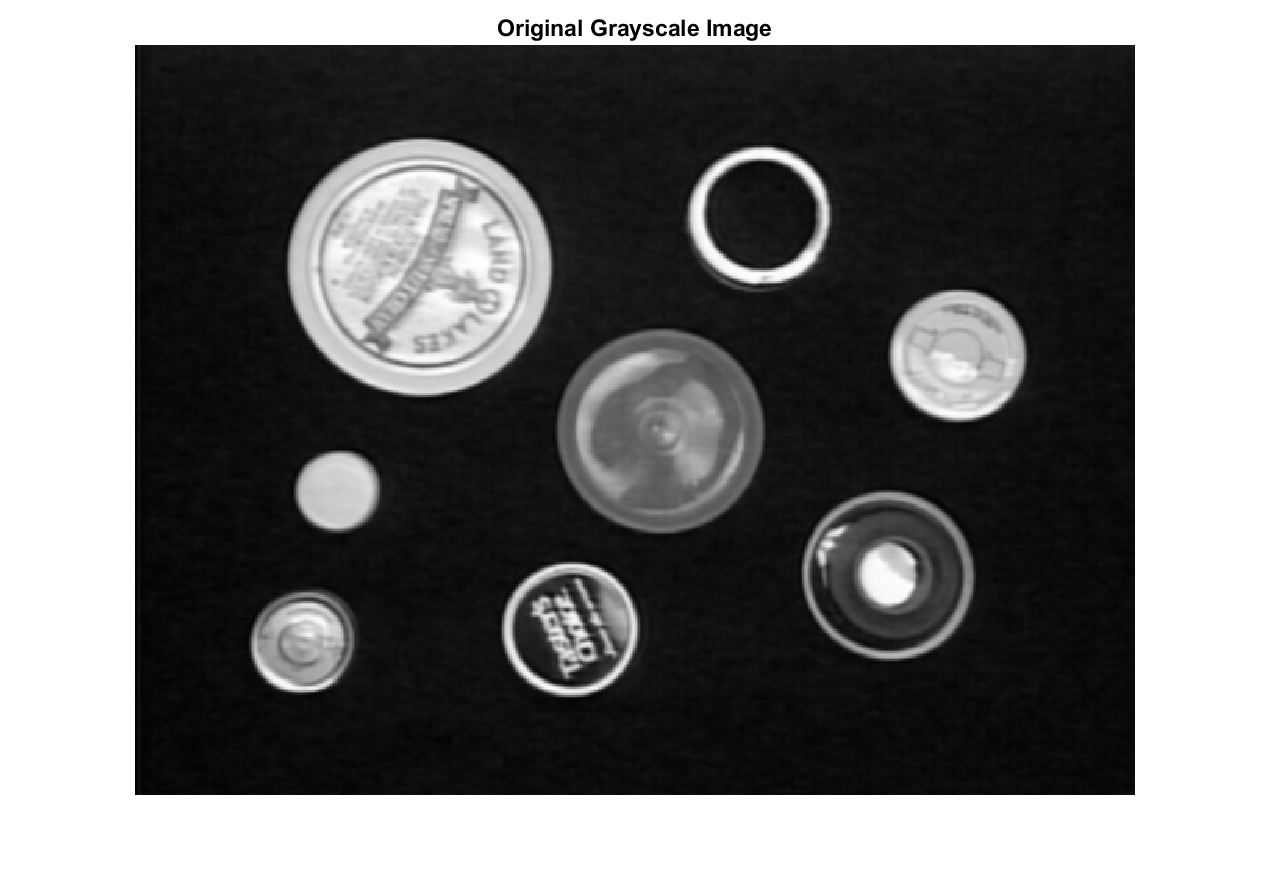
\includegraphics[width=0.7\linewidth]{original_grayscale_image}
	\caption{Part 5 - Original Grayscale Image $\sigma$ = 1 w. Gaussian Filter }
	\label{fig:originalgrayscaleimage}
\end{figure}

\begin{figure}
	\centering
	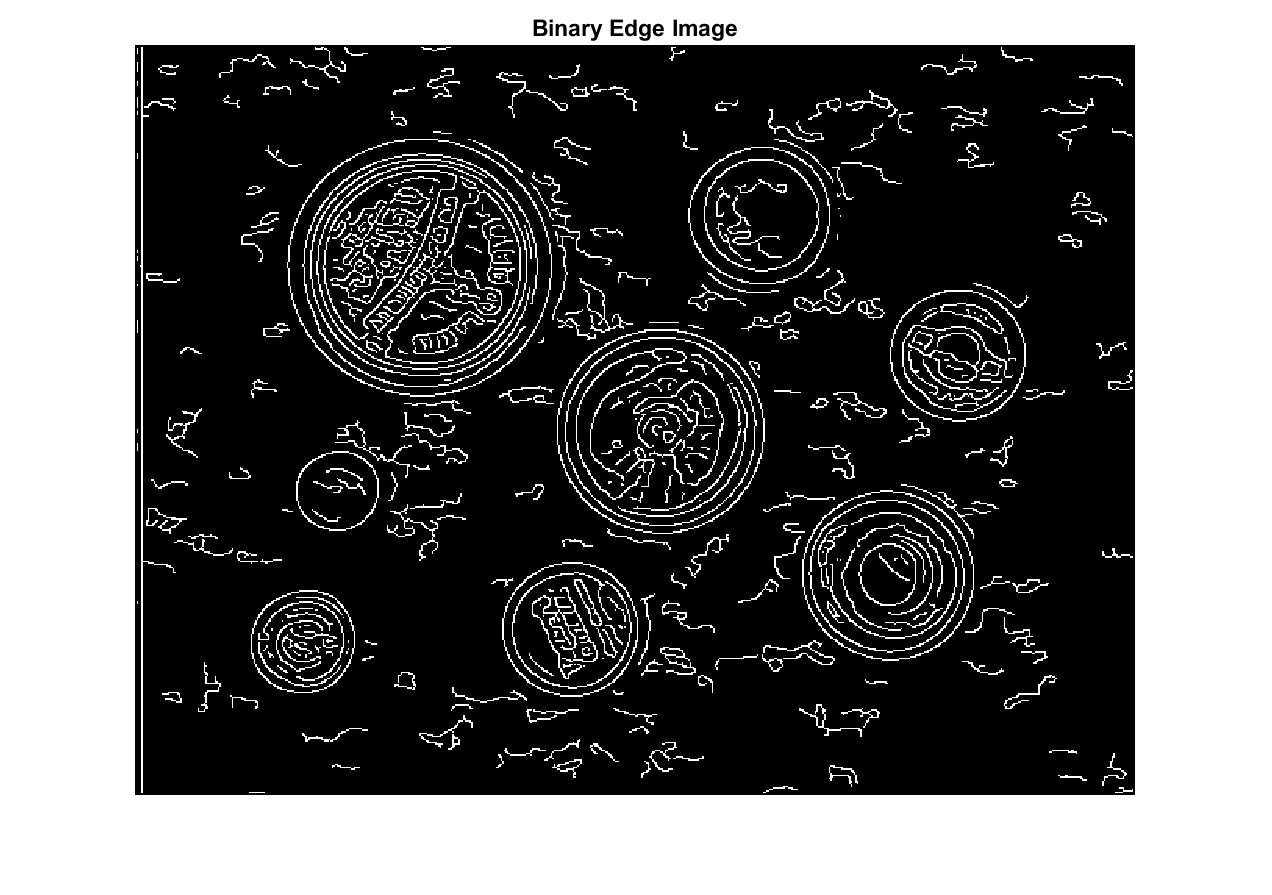
\includegraphics[width=0.7\linewidth]{binary_edge_image}
	\caption{Part 5 - Binary Edge Image $\sigma$ = 1 w. Gaussian Filter}
	\label{fig:binaryedgeimage}
	
\end{figure}


\begin{figure}
	\centering
	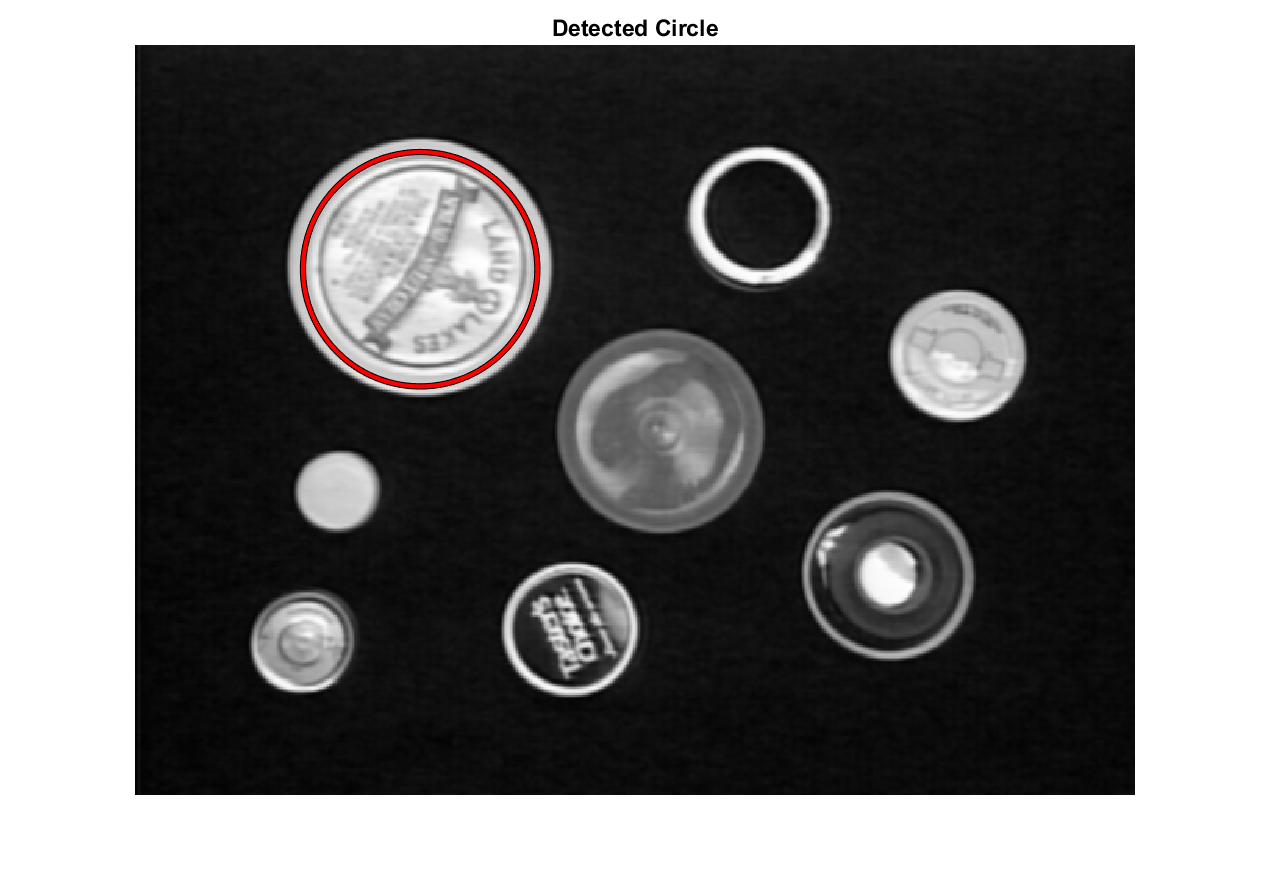
\includegraphics[width=0.7\linewidth]{detected_circle}
	\caption{Part 5 - Original image with detected dominant circle superimposed on it}
	\label{fig:detectedcircle}
	
	\begin{tabular}{|c|}
		\hline
		\\
		\hline
		Detected circle parameters: \\
		\hline
		Center: (183, 144) \\
		\hline
		Radius: 75 \\
		\hline
		Hough Space maximum value: 223 \\
		\hline
		Hough Space maximum location: (183, 144, 12) \\
		\hline
		Hough Space size: 640 x 480 x 17 \\
		\hline
	\end{tabular}
	
\end{figure}

\begin{figure}
	\centering
	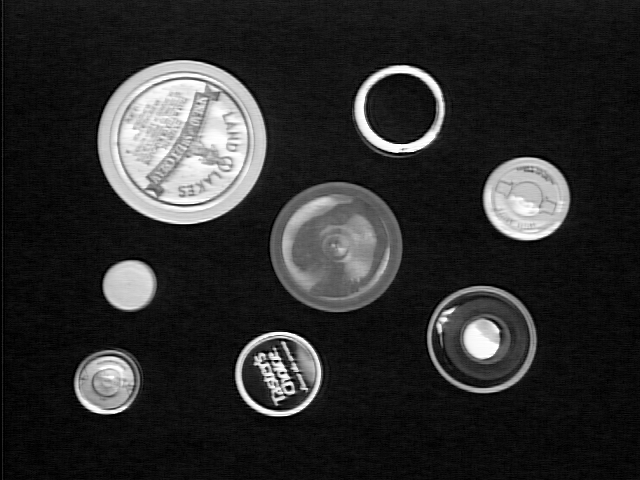
\includegraphics[width=0.7\linewidth]{original_grayscale_image_2024-02-17_140115}
	\caption{Part 6- Original Grayscale Image $\sigma$ = 1 w. Gaussian Filter }
	\label{fig:originalgrayscaleimage2024-02-17140115}
\end{figure}
\begin{figure}
	\centering
	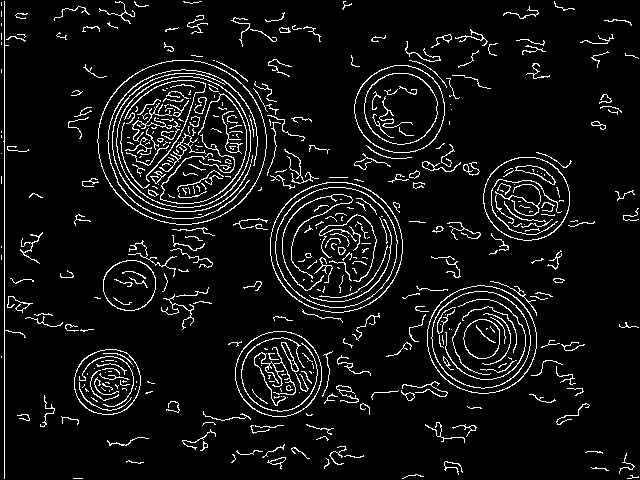
\includegraphics[width=0.7\linewidth]{binary_edge_image_2024-02-17_140115}
	\caption{Part 6 - Binary Edge Image $\sigma$ = 1 w. Gaussian Filter}
\end{figure}
\begin{figure}
	\centering
	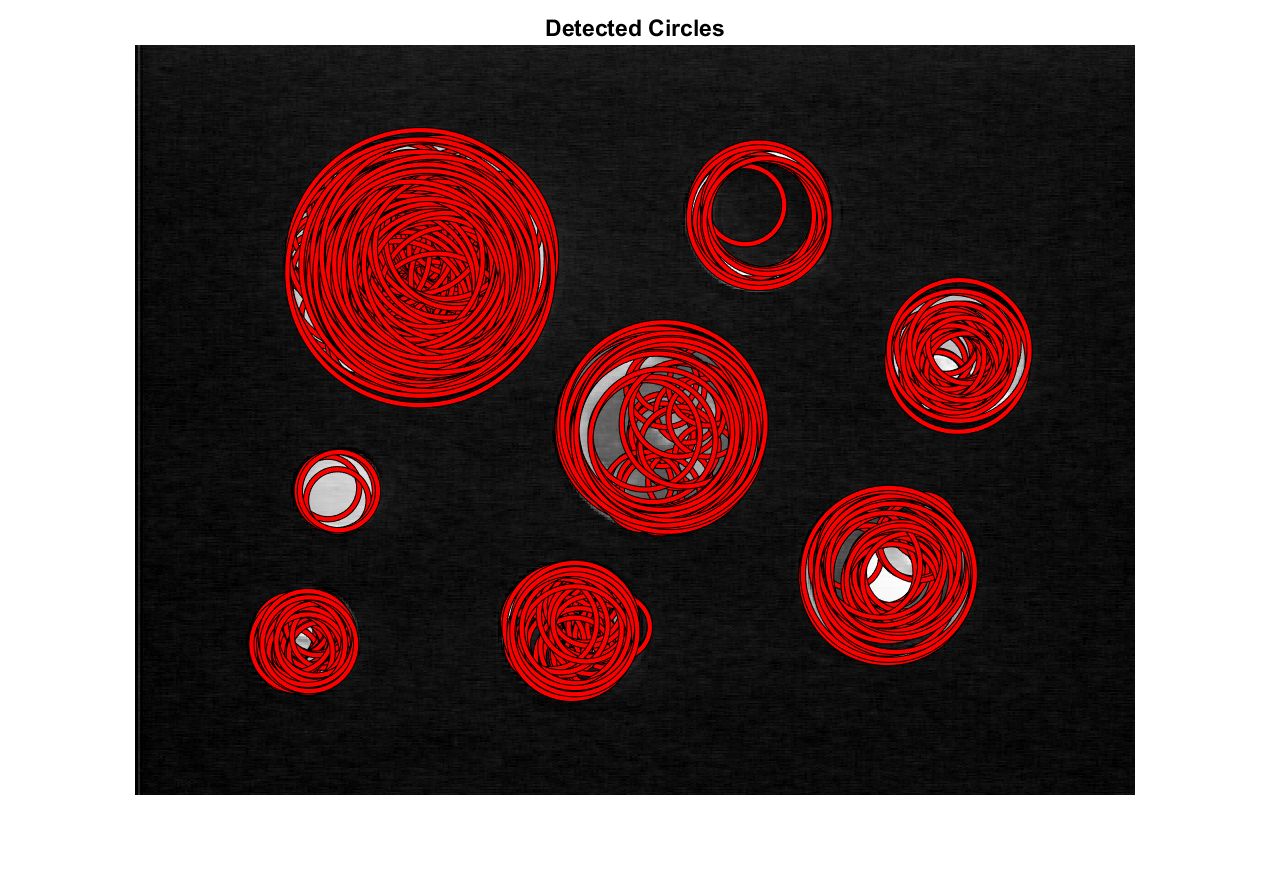
\includegraphics[width=0.7\linewidth]{all_detected_circles_2024-02-17_140115}
	\caption{Part 6- All detected circles Threshold = 0.5}
	\label{fig:alldetectedcircles2024-02-17140115}
\end{figure}
\begin{figure}
	\centering
	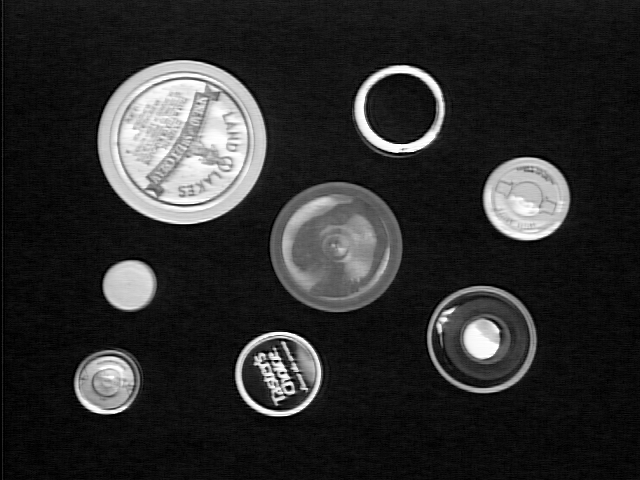
\includegraphics[width=0.7\linewidth]{original_grayscale_image_2024-02-17_142108}
	\caption{Part 6- Original Grayscale Image $\sigma$ = 1 w. Gaussian Filter}
	\label{fig:originalgrayscaleimage2024-02-17142108}
\end{figure}

\begin{figure}
	\centering
	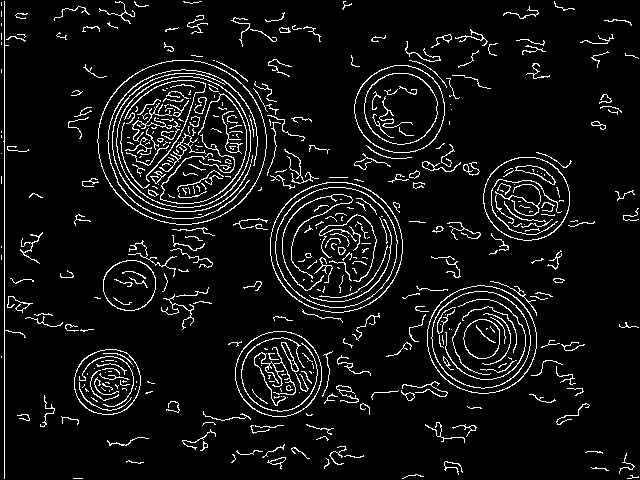
\includegraphics[width=0.7\linewidth]{binary_edge_image_2024-02-17_142108}
	\caption{Part 6 - Binary Edge Image $\sigma$ = 1 w. Gaussian Filter}
	\label{fig:binaryedgeimage2024-02-17142108}
\end{figure}
\begin{figure}
	\centering
	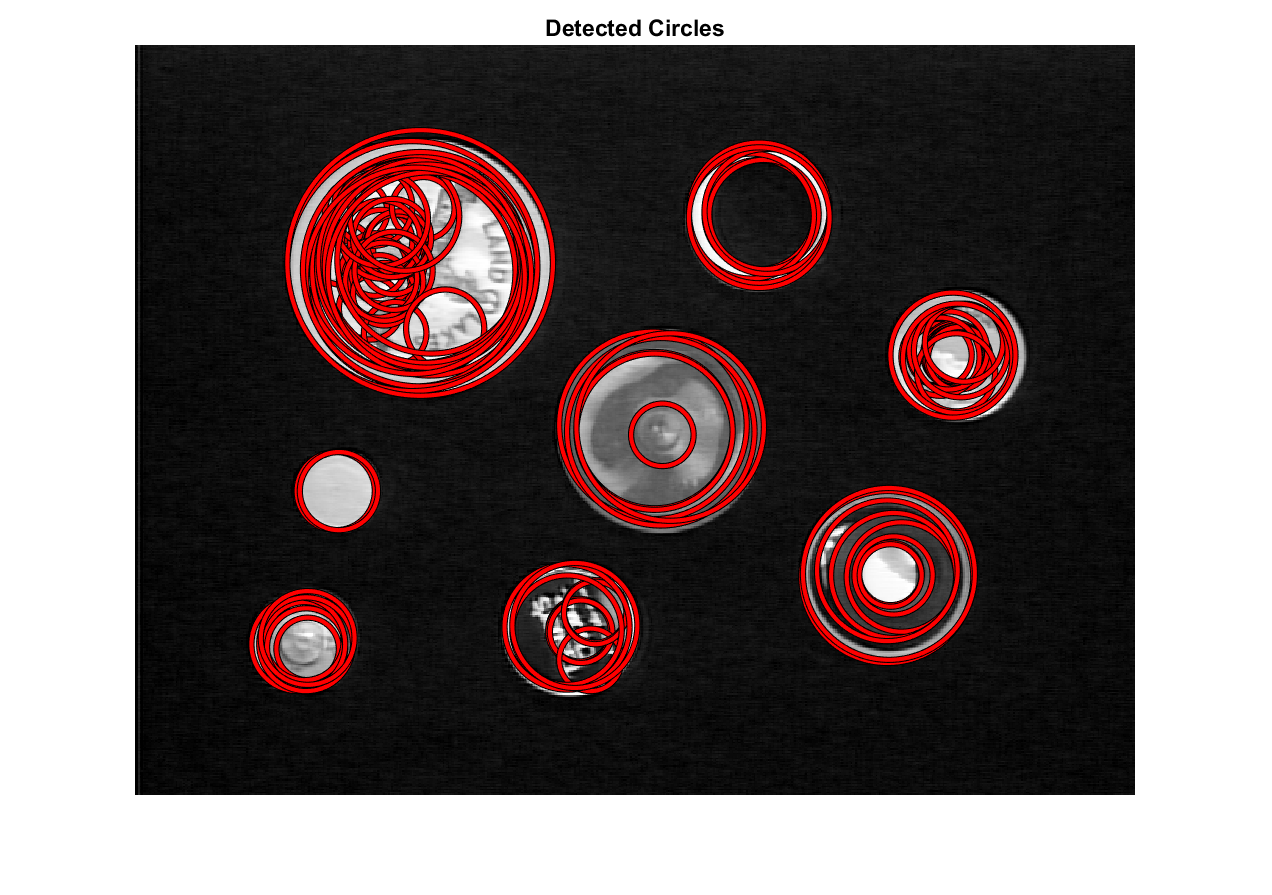
\includegraphics[width=0.7\linewidth]{all_detected_circles_2024-02-17_142108}
	\caption{Part 6 - All Detected Circles. A threshold value of $0.6 \times \max(\text{HoughSpace})$ was used to identify the most prominent circles in the image. This higher threshold ensures that only the most significant accumulations in the Hough Space, which correspond to strong circle candidates, are considered for detection.}
	\label{fig:alldetectedcircles2024-02-17142108}
\end{figure}
\cleardoublepage
\part{A list of the parameters of the detected circles Threshold value of $0.6 \times \max(\text{HoughSpace})$ }

\cleardoublepage



\begin{tabular}{|c|c|c|}
	
	\hline
	Center\_X & Center\_Y & Radius \\
	\hline
	111 & 387 &20 \\
	\hline
	133& 134& 20 \\
	\hline
	142& 107& 20 \\
	\hline
	151& 169& 20 \\
	\hline
	154& 141& 20 \\
	\hline
	157& 155& 20 \\
	\hline
	158& 126& 20 \\
	\hline
	159& 146& 20 \\
	\hline
	160& 160& 20 \\
	\hline
	166& 140& 20 \\
	\hline
	167& 129& 20 \\
	\hline
	167& 185& 20 \\
	\hline
	168& 129& 20 \\
	\hline
	169& 127& 20 \\
	\hline
	185& 105& 20 \\
	\hline
	285& 375& 20 \\
	\hline
	285& 376&20 \\
	\hline
	286& 376& 20 \\
	\hline
	292& 394& 20 \\
	\hline
	295& 363&20 \\
	\hline
	295& 364& 20 \\
	\hline
	338& 250& 20 \\
	\hline
	484& 339& 20 \\
	\hline
	484& 340& 20 \\
	\hline
	516& 199& 20 \\
	\hline
	525& 198& 20 \\
	\hline
	525& 199& 20 \\
	\hline
	526& 200& 20 \\
	\hline
	527& 200& 20 \\
	\hline
	527& 201& 20 \\
	\hline
	528& 201& 20 \\
	\hline
	109& 382& 25 \\
	\hline
	110& 386& 25 \\
	\hline
	129& 286& 25 \\
	\hline
	131& 286& 25 \\
	\hline
	153& 104& 25 \\
	\hline
	156& 150& 25 \\
	\hline
	158& 125& 25 \\
	\hline
	160& 152& 25 \\
	\hline
	165& 124& 25 \\
	\hline
	166& 145& 25 \\
	\hline
	199& 182& 25 \\
	\hline
	486& 340& 25 \\
	\hline
	516& 200& 25 \\
	\hline
	521& 196& 25 \\
	\hline

\end{tabular}
\begin{tabular}{|c|c|c|}
	\hline
	Center\_X & Center\_Y & Radius \\
\hline
526& 210& 25 \\
\hline
531& 191& 25 \\
\hline
105& 384& 30 \\
\hline
110& 384&30 \\
\hline
111& 380& 30 \\
\hline
158& 112& 30 \\
\hline
529& 196& 30 \\
\hline
173& 110& 35 \\
\hline
277& 375& 35 \\
\hline
400& 109& 35 \\
\hline
403& 109& 35 \\
\hline
491& 341& 35 \\
\hline
527& 201& 35 \\

277&373& 40 \\
\hline
282& 372& 40 \\
\hline
395& 110& 40 \\
\hline
405& 107& 40 \\
\hline
486& 340& 40 \\
\hline
524& 199& 40 \\
\hline
400& 108& 45 \\
\hline
400& 111& 45 \\
\hline
482& 337& 45 \\
\hline
333& 247& 50 \\
\hline
333& 248& 50 \\
\hline
482& 341& 55 \\
\hline
483& 339& 55 \\
\hline
190& 138& 60 \\
\hline
332& 244& 60 \\
\hline
337& 248& 60 \\
\hline
343& 245& 60 \\
\hline
179& 146& 65 \\
\hline
182& 142& 65 \\
\hline
183& 139& 65 \\
\hline
186& 139& 65 \\
\hline
187&142& 65 \\
\hline
189& 147& 65 \\
\hline
179& 141& 70 \\
\hline
180& 149& 70 \\
\hline
183& 144& 75 \\
\hline
178& 142& 80 \\
\hline
183& 140& 85 \\
\hline


\end{tabular}

\end{document}

